\section{Methodology}

We intend to utilize the following methods:
\begin{itemize}
    \item[--] Exploratory analysis
    \item[--] Regression, https://www.alchemer.com/resources/blog/regression-analysis/
    \item[--] ARIMA, https://www.machinelearningplus.com/time-series/arima-model-time-series-forecasting-python/
    \item[--] LSTM --- Tensorflow
    \end{itemize}

\subsection{Data gathering}
In order to analyze data connected to salmon price, we first need to gather this data. 
The main data point is the price of salmon. There are several sources for this data, but we utilized the data from the NASDAQ salmon exchange.
The reason for this being a combination of the accessibility of the data, and the fact that the NASDAQ salmon exchange (NQSALMON)
uses a wighted average for the salmon price, gathered from a spectrum of salmon exporters and it is therefore the best source of meaningful data.
Another reason for using the NASDAQ salmon exchange is that the data is updated weekly with no missing values for the entire time frame.
We downloaded data from March 2013 through December 2022, for a total of 507 data points. This was our base for the independent factors.

The next step was to gather data from the other relevant factors for our analysis. 


\subsection{Exploratory analysis}

\subsection{ARIMA and SARIMAX}

As explained in~\ref{SeasonalityTheory} on page~\pageref{SeasonalityTheory}, one of the prerequisites for the ARIMA model is that the data is stationary. This can be done either by analysing the time-series itself and noticing the variance and trend, or by using the Augmented Dickey-Fuller test. 
After this is done, the next step will be to find the optimal parameters for the ARIMA model. This is usually done by looking at the ACF and PACF plots. 
When the optimal parameters are found, the model can be fitted and used to predict future values. \parencite{hyndman_athanasopoulos_2021}

\subsubsection{Stationarity}
The Augmented Dickey-Fuller test is a statistical test that can be used to determine stationarity. The null hypothesis of the test is that the time-series is non-stationary. If the p-value is less than the significance level, the null hypothesis is rejected and the time-series is expected to be stationary.
Using the Augmented Dickey-Fuller test on the Salmon Price data, we get a p-value of 0.05651, this means that we cannot reject the null hypothesis at a 95\% confidence level. The data is therefore not stationary.~\parencite{Dickey_Fuller1979}

In order to better understand why the data is not stationary, we can plot the data and look at the variance, trend and seasonality. This is done by decomposing the data into its components. We then get the following plot: 

\begin{figure}[H]
    \centering
    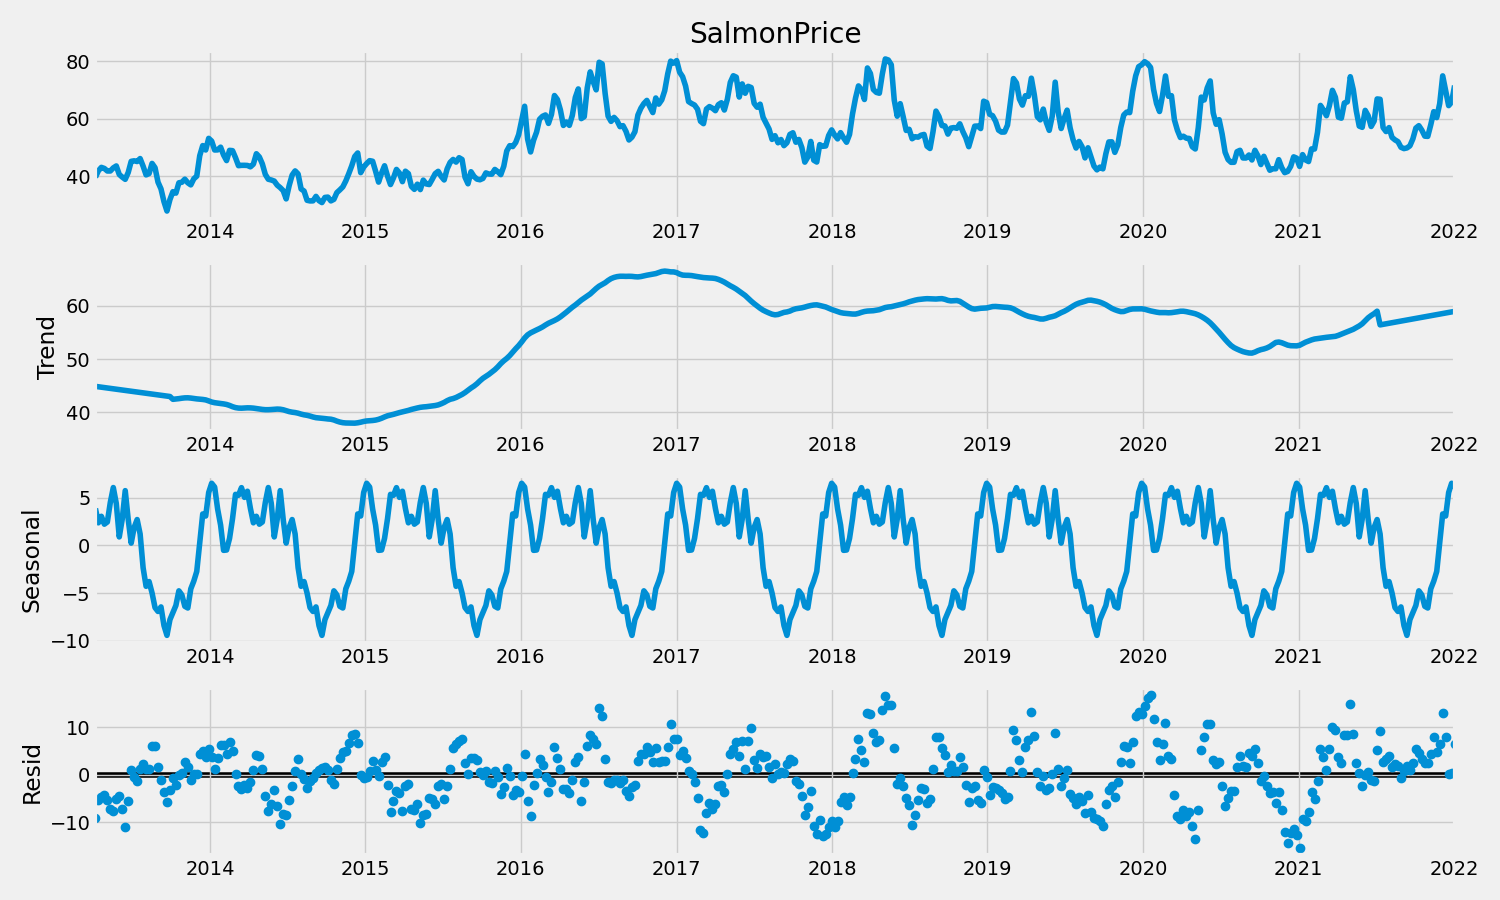
\includegraphics[width=0.8\textwidth]{data/Figures/ARIMA/Decomposition.png}
    \caption[Decomposition of the Salmon Price data]{Decomposition of the Salmon Price data.}\label{fig:Decomposition}
\end{figure}
Examining the decomposed data there are especially two things that stand out. The first is the trend, which is clearly increasing. The second is the seasonality, there is a clear yearly seasonal trend where the price is higher in the summer months before decreasing during the autumn and reaching a low in the winter. From this we can draw the same conclusion as the Augmented Dickey-Fuller test, the data is not stationary and needs differencing. In the ARIMA model, this will be done by setting $d$ to 1 or more. 

The exact number of differencing needed can be found either by using the ADF-test on the differenced data and looking for when the p-value is less than the critical value, or by looking at the ACF and PACF plots. 

\subsection{LSTM --- Tensorflow}